\section{Specifics of the protocol settings and visual stimuli}
\label{sec:Specifics-of-the-protocol-settings-and-visual-stimuli}

In a session, the three stimuli presentation protocols were ordered as RF mapping, tuning mapping and then the actual SM examination.
Each protocol is associated with different stimuli characteristics, specific to the controls or information that were to be required from the final extracted data. Furthermore, each kind of protocol had also distinct specifications in regards to the time durations in the trial structure of the session.
The mice were always placed with their right eye parallel and at $15 cm$ from the center of the monitor. All of the stimuli measurements will thus follow indicated in degrees at the mice's perspective to the screen, in azimuth (horizontal axis) and in elevation (vertical axis) coordinates. In addition, to compensate for the screen's flatness, spherical corrections were applied to the displayed stimuli, so that what the mice visualized corresponded to the same size of stimuli at each patch location, irrespective of its distance in the screen and that no distortions in the gratings were perceived by the animal.
Every protocol underwent pseudorandomization of the trials: Each type of trial appeared the same number of N repetitions, but at shuffled order. The reason for this was to minimize the neurons adaptation [REFERENCES] to the specific trial types, as they had to be repeated a reasonable amount of times for significant analysis.

\subsection{Receptive Field mapping stimuli}
\label{subsec:subasectionC}

This protocol consisted on the presentation of a 10º squared cell (in the mouse's referential) with a small moving bar inside. At each trial, this bar moved in four directions, in sequence but at random order - bottom to top (labelled 0º), left to right (90º) and the opposite ones (180º and 270º, respectively). The moving bar had $4º$ width and $25 º/s$ speed, with the dark at $0 WHAT$, the light at $204 WHAT$ and the background at $102 WHAT$. This patch appeared in any of 80 positions in the monitor, which was divided in a $10 \times 10$ grid, tiling a circle with 50º maximum radius from the center. The presentation was repeated in each grid position 14 times, to a total of 1120 trials, at shuffled order whithin each repetition.

At each trial of $1 s$, the stimulus played for $220 ms$ and was followed by an $880ms$ ITI, summing 19 minutes of RF mapping at each session. 

 \begin{table}[H]
\begin{center}\par
\scalebox{0.85}{
\begin{tabular}{c|cccccccccccccccccccccccccc}
\hline 
 
    
\multicolumn{1}{c}{Feature} & Value \\
           
           \hline
           \hline

\multicolumn{1}{c}{cell size (º)} & 10 \\
\multicolumn{1}{c}{cell grid (º)} & [10, 10] \\
\multicolumn{1}{c}{maximum radius (º)} & 50 \\
\multicolumn{1}{c}{stim directions (º)} & [0 90 180 270] \\
\multicolumn{1}{c}{bar width (º)} & 4 \\
\multicolumn{1}{c}{bar speed (º/s)}& 10 \\
\multicolumn{1}{c}{dark, stim, background light} & [0 204 102] \\
\hline
        
\end{tabular}}
 \caption{Configurations regarding the RF mapping protocol stimuli properties.}
    \vspace{-5mm}
    \label{table:RF}
\end{center}
\end{table}

\begin{figure}[H] \centering 
\includegraphics[width=10cm,height=10cm,keepaspectratio]{Figures/4.Chapter/rf.png} \caption{rf example.} \end{figure}

\subsection{Tunings mapping stimuli}
\label{subsec:subbsectionC}

The selectivity of each neuron was also controlled for spatial and temporal frequencies, as well as for more gratings' directions of movement. 

With the same contrast configurations as for the previous protocol, a circular centered patch of $30º$ was presented at any of 8 directions: the previous and the intermediatedly oriented ones ($0º$, $45º$, $90º$, $135º$, $180º$, $225º$, $270º$ and $315º$). The gratings could have $0.02 /º$ or $0.04 /º$ of spatial frequency and $0.5 Hz$ or $1 Hz$ as temporal frequency. Together, each of these 32 configurations of direction and frequencies were presented in 25 repetitions, totaled at 800 trials and shuffled within the full protocol.

Each trial had $1 s$, divided in a baseline of $5 ms$, a stimulus presentation of $900 ms$ and an ITI of $95 ms$, to a total of 14 minutes per session.

\begin{table}[H]
\begin{center}\par
\scalebox{0.85}{
\begin{tabular}{c|cccccccccccccccccccccccccc}
\hline 
 
    
\multicolumn{1}{c}{Feature} & Value \\
           
           \hline
           \hline

\multicolumn{1}{c}{stimulus size (º)} & 30 \\
\multicolumn{1}{c}{stimulus center (º)} & [0, 0] \\
\multicolumn{1}{c}{stim directions (º)} & [0 45 90 135 180 225 270 315] \\
\multicolumn{1}{c}{spatial frequency (/º)} & [0.02 0.04] \\
\multicolumn{1}{c}{temporal frequency (Hz)}& [0.5 1] \\
\multicolumn{1}{c}{dark, stim, background light} & [0 204 102] \\
\hline
        
\end{tabular}}
 \caption{Configurations regarding the tuning mapping protocol stimuli properties.}
    \vspace{-5mm}
    \label{table:tuning}
\end{center}
\end{table}

\begin{figure}[H] \centering 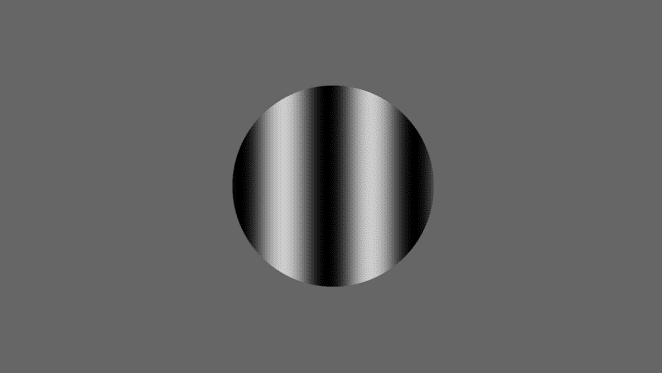
\includegraphics[width=4cm,height=4cm,keepaspectratio]{Figures/4.Chapter/tuning.png} \caption{tuning example.} \end{figure}

\subsection{Surround Modulation stimuli}
\label{subsec:subcsectionC}

Finally, for the SM protocol the frequencies of $0.04 /º$ and $1 s$ were chosen based on previous reports of largest V1 stimulation [REFERENCES]. The light contrasts of the gratings went from $0$ at dark to $122.5$ at background and $255$ at the lightest. Each trial had $2 s$, with $0.5 s$ of baseline, $1 s$ of stimuli display and $0.5 s$ of ITI. 

There were 124 possible trial types, repeated 20 times, to a total of 2480 trials in an 1 hour and 23 minutes session.

 \begin{table}[H]
\begin{center}\par
\scalebox{0.85}{
\begin{tabular}{c|cccccccccccccccccccccccccc}
\hline 
 
    
\multicolumn{1}{c}{Feature} & Value \\
           
           \hline
           \hline

\multicolumn{1}{c}{spatial frequency (/º)} & 0.04 \\
\multicolumn{1}{c}{temporal frequency (Hz)} & 1 \\

\multicolumn{1}{c}{central radius (º)} & 15 \\
\multicolumn{1}{c}{surround inner and outer radius (º)} & [27 50] \\
\multicolumn{1}{c}{stim directions (º)} & [0 90 180 270] \\
\multicolumn{1}{c}{dark, stim, background light} & [0 255 122.5] \\
\multicolumn{1}{c}{groups of stimuli} & C, S1, S1+C, S2, S2+C \\
\hline
        
\end{tabular}}
 \caption{Configurations regarding the SM protocol stimuli properties.}
    \vspace{-5mm}
    \label{table:SM}
\end{center}
\end{table}

There were 5 possible patches: a central one and four surround patches in the cardinal positions. The central patch was a circle of 15º radius, as the others were limited by an external circumference of 50º, an inner circumference of 27º (to obtain a 12º gap between the center and the surround patches) and the curresponding bissectors of the screen. For any patch, there were 4 available directions of gratings movement ($0º$, $90º$, $180º$ and $270º$).

With these patches, five groups of stimuli types were used:
\begin{itemize}
\item $C$ - only the center patch, in any of the 4 directions of movement (4 types);

\begin{figure}[h]\centering 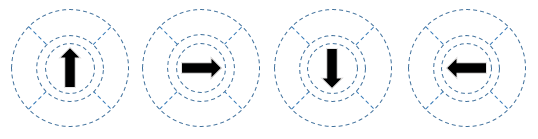
\includegraphics[width=9cm,height=9cm,keepaspectratio]{Figures/4.Chapter/C.PNG} \caption{Diagram of stimuli group C.} \end{figure}

\item $S1$ - only one surround patch, in any of the 4 cardinal top, bottom, left or right locations (S1T, S1B, S1L, S1R), and in any of the 4 directions (16 types);

\begin{figure}[h]\centering 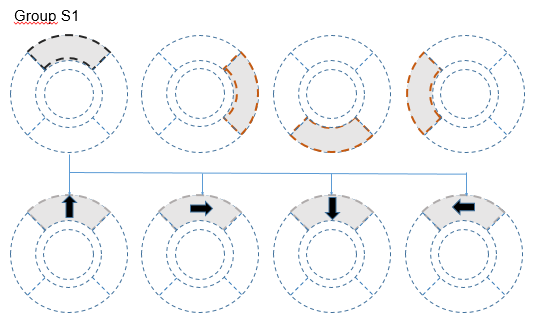
\includegraphics[width=9cm,height=9cm,keepaspectratio]{Figures/4.Chapter/S1.PNG} \caption{Diagram of stimuli group S1.} \end{figure}

\item $S1+C$ - One surround patch and the center patch, at any location of the surround($S1T+C$, $S1B+C$, $S1L+C$, $S1R+C$) and any direction for the center and for the surround (64 types);

\begin{figure}[H] \centering 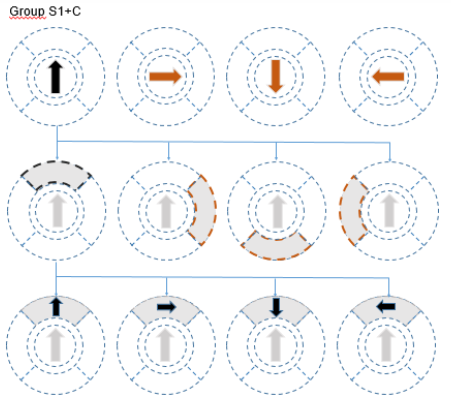
\includegraphics[width=9cm,height=9cm,keepaspectratio]{Figures/4.Chapter/S1C.PNG} \caption{Diagram of stimuli group S1C.} \end{figure}

\item $S2$ - only two surround patches, in opposite cardinal locations, either in the horizontal line ($S2H$) or the vertical line ($S2V$), both of them with gratings moving in the same of any of the 4 directions (8 types);

\begin{figure}[H] \centering 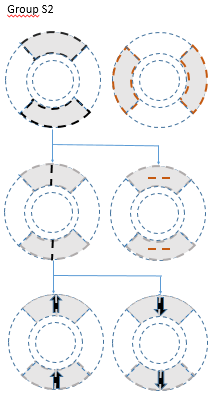
\includegraphics[width=8cm,height=8cm,keepaspectratio]{Figures/4.Chapter/S2.PNG} \caption{Diagram of stimuli group S2.} \end{figure}

\item $S2+C$ - Two surround patches and the center patch, both surround patches either in the horizontal ($S2H+C$) or the vertical line ($S2V+C$), both with gratings moving in the same of the possible directions and the center patch with gratings moving in any direction, not necessarily being the same from the surround stimuli (32 types).

\begin{figure}[H] \centering 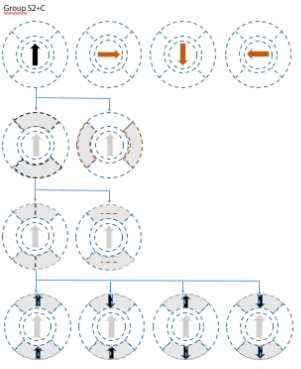
\includegraphics[width=10cm,height=10cm,keepaspectratio]{Figures/4.Chapter/S2C.PNG} \caption{Diagram of stimuli group S2C.} \end{figure}

\end{itemize}


\begin{figure}[H] \centering 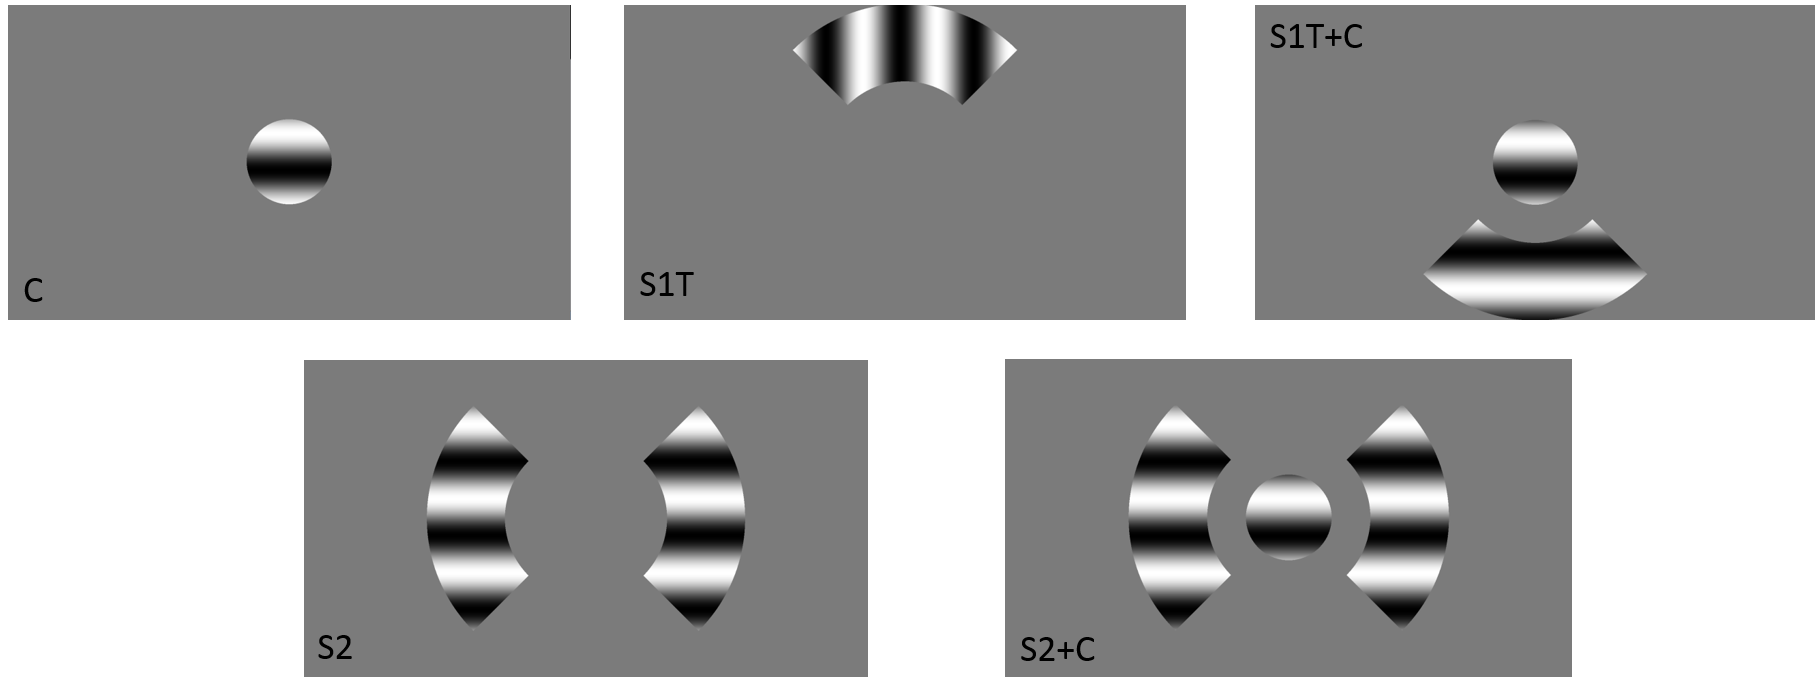
\includegraphics[width=12cm,height=12cm,keepaspectratio]{Figures/4.Chapter/SM.png} \caption{SM examples.} \end{figure}

Group $C$ was used as a more specific confirmation for the receptive field findings: here the stimuli was now in the center of the screen with the selected size for the analysis. Groups $S1$ and $S2$ provided the data that allowed to exclude from the analysis the cells that responded to stimulation in the defined surround. These had a receptive field that overlapped what we regarded as the surround and thus did not meet the criteria for investigating surround modulation effects in this experiment's designed manner. With the cells that did respond to group $C$ but did not to group $S1$ nor $S2$, we could then regard the effects of actual surround stimulation by examinating the responses to stimuli in the groups $S1+C$ and $S2+C$.